\documentclass[10pt,aspectratio=43]{beamer}

\usepackage{graphicx}
\usepackage{tikz}
\usepackage{xcolor}
\usepackage{caption}
\usepackage{subcaption}
\usepackage{bm}
\usetikzlibrary{calc} 
\usepackage{hyperref}
\hypersetup{
    colorlinks=true,
    linkcolor=blue,
    urlcolor=red
}
\usepackage{fontawesome5}
\usepackage{ulem}
\usepackage{wasysym}

\usetheme{MyStyle}   % loads beamerthemeMyStyle.sty
\setlength{\columnsep}{0pt}


%%%%%%%%%%%%%%%%%%%%%%%%%%%%%%%%%%%%%%%%%%
%%%%%%%%%%%%%%%%%%%%%%%%%%%%%%%%%%%%%%%%%%
%%%%%%%%%%%%%%%%%%%%%%%%%%%%%%%%%%%%%%%%%%

\title{ALERT AHDC tracking \\ and alignment}
\newcommand{\eventname}{CLAS Collaboration meeting}
\author{Felix Touchte Codjo}
\institute{IJCLab}
%\date{\today}
\date{June 30, 2026}


\begin{document}

\begin{frame}[plain] % remove header, footer, barre de navigation
\titlepage
\end{frame}

% \begin{frame}{Outline}
% \tableofcontents
% \end{frame}

%\section{Intro}
%\section{Updates}

% \begin{frame}{The ALERT detector}
%     \begin{itemize}
%         \item 
%     \end{itemize}
    
% \end{frame}

\begin{frame}{ALERT alignment status}
    
    \begin{itemize}
        \item Layer alignment (before, after, correction angles)
    \end{itemize}

    {
    \setlength{\tabcolsep}{3pt}
    \begin{tabular}{ccc}
        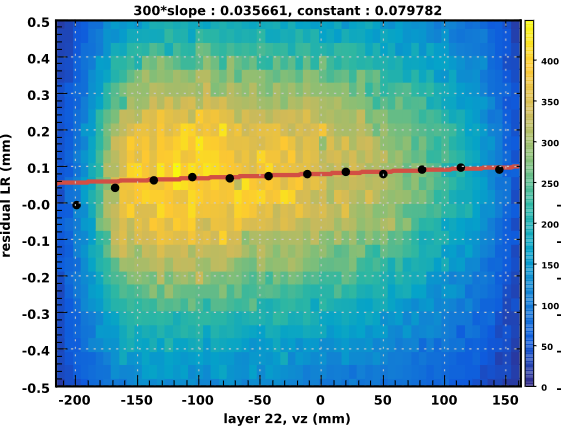
\includegraphics[width=0.32\linewidth]{figures/layer22_without_alignment.png} &
            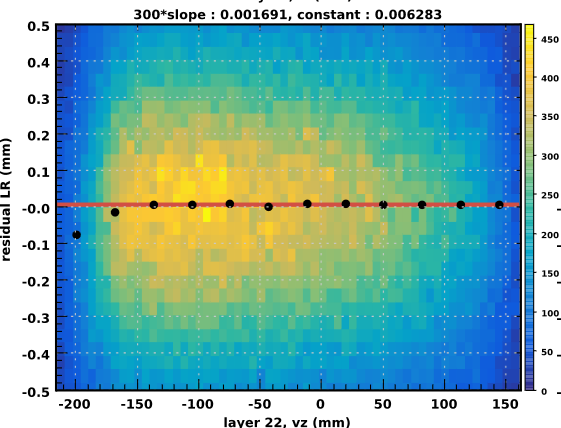
\includegraphics[width=0.32\linewidth]{figures/layer22_with_alignment.png} &
            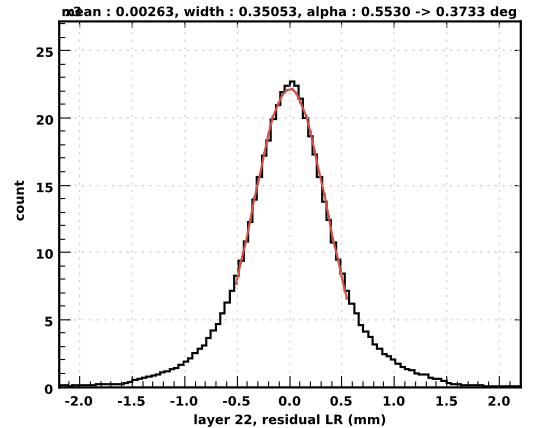
\includegraphics[width=0.32\linewidth]{figures/layer22_alignment_angles.png}
    \end{tabular}
    }
    

    \begin{minipage}{0.5\linewidth}
        \begin{itemize}
            \item vz alignment with respect to CLAS
        \end{itemize}

        \begin{figure}
            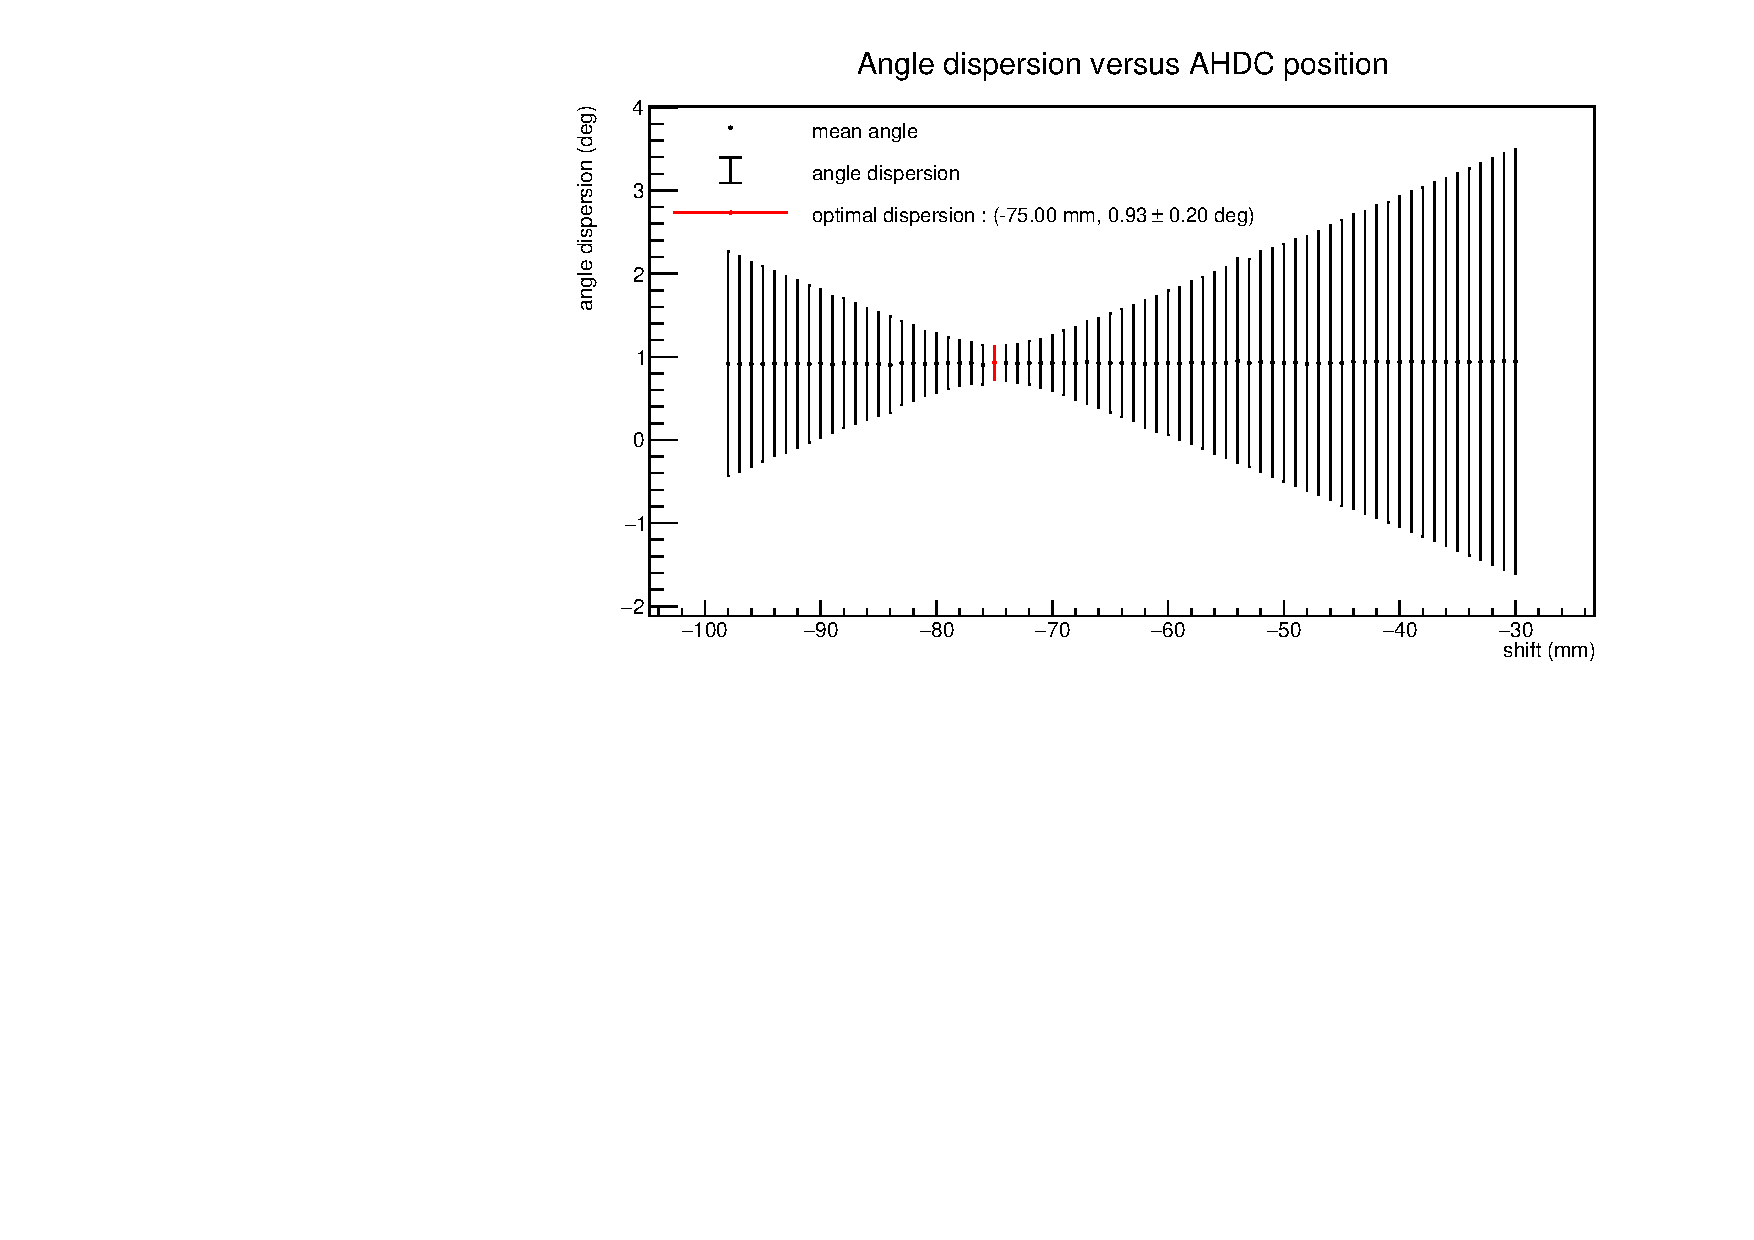
\includegraphics[width=\linewidth]{figures/ahdc_position_scan.pdf}
        \end{figure}
    \end{minipage}
    \begin{minipage}{0.46\linewidth}
        \begin{itemize}
            \item Summary
                \begin{itemize} 
                    \setlength{\leftskip}{-0.5cm}
                    \footnotesize
                    \item The layer alignment applies correction angles (rotZ) to the upstream and downstream ends of the AHDC
                    \item The wire by wire alignment remains to be done
                    \item The vz alignment with respect to CLAS has been done on 2 GeV runs, it needs to be done for 10.6 GeV runs (ongoing task)
                \end{itemize}
        \end{itemize}
    \end{minipage}

\end{frame}


\end{document}


